%!TEX root = book.tex

\chapter{Problem Sets}

%\setcounter{secnumdepth}{1}

\clearpage
\problemset

\begin{problem}
In the Schwarzschild metric, the frequency of a photon varies such that
$h\nu(1-2GM/c^2r)^{1/2}$ is constant \cite*[p.\ 187 and p.\ 659,
  although note that these authors set $G = c = 1$]{Misner-1973}.
\begin{enumerate}
\item[(a)]
Calculate the gravitational redshift $z \equiv \Delta\nu/\nu$ from the bottom to the top of the solar atmosphere. Assume that the thickness of the solar atmosphere is 600 km.
\item[(b)] Most computer programs used to model stellar atmospheres use
  single-precision floating-point numbers that typically are precise to
  about $10^{-7}$. Which is likely to lead to larger errors, using this
  representation or ignoring the gravitational redshift across the solar
  atmosphere?
\label{problem-gravitational-redshift}
\end{enumerate}
\end{problem}

%\begin{problem}
%\label{problem-photon-density}
%\label{problem-energy-density}
%Show that in general (a) the total density of photons is $(4\pi/h c)
%\int_0^\infty\!d\nu\: J_\nu / \nu$ and (b) the total energy density is
%$4\pi J / c$.
%\end{problem}

\begin{problem}
Consider a solid sphere whose surface emits with uniform specific
intensity $I$ outwards into empty space. 
\begin{enumerate}
\item[(a)]
Use the constancy of specific
intensity to show that the flux from the sphere drops according to the
inverse square law. 
\item[(b)] What is the flux at the surface? 
\end{enumerate}

\end{problem}

%\begin{problem}
%\label{problem-flux-from-surface}
%If $I_\nu$ is
%isotropic over the outward hemisphere and zero over the
%inward hemisphere, i.e.,
%\begin{align}
%I_\nu(\mu) =
%\begin{cases}
%I_\nu(1)&\mbox{for $\mu>0$,}\\
%0&\mbox{for $\mu<0$,}
%\end{cases}
%\end{align}
%where $I_\nu(1)$ is a constant, 
%show that
%\begin{align}
%F_\nu = \pi I_\nu(1).
%\end{align}
%\end{problem}

%\begin{problem}
%\label{problem:f-with-odd-function}
%
%% If $I(\mu)$ has the form
%% \begin{align}
%% I_\nu(\mu) = 
%% \begin{cases}
%% I^+_0 + \sum_{i=0}^\infty I_{2i+1} \mu^{2i+1}&\mbox{for $\mu \ge 0$,}\\
%% I^-_0 + \sum_{i=0}^\infty I_{2i+1} \mu^{2i+1}&\mbox{for $\mu <   0$,}
%% \end{cases}
%% \end{align}
%% show that Eddington factor $f \equiv K_\nu/J_\nu$ is
%% $1/3$. This is a generalization of the result for an
%% isotropic radiation field.
%% \end{problem}
%%
%% Roberto Galván suggested the following more elegant version.
%
%If $I(\mu)$ has the form
%\begin{align}
%I_\nu(\mu) = 
%\begin{cases}
%I_0 + g(+\mu)&\mbox{for $\mu \ge 0$,}\\
%I_0 - g(-\mu)&\mbox{for $\mu <   0$,}
%\end{cases}
%\end{align}
%show that Eddington factor $f \equiv K_\nu/J_\nu$ is $1/3$. (This is
%a generalization of the result for an isotropic radiation field; if one
%adds an odd component to an isotropic radiation field, the Eddington
%factor remains $1/3$.)
%\end{problem}

%\begin{problem}
%\label{problem-eddington-factor-range}
%The Eddington factor is defined by $f \equiv K_\nu/J_\nu$.
%\begin{enumerate} 
%\item[(a)]
%Show that $0 \le f \le 1$ provided $f$ is well defined (i.e., $J_\nu
%> 0$).
%\item[(b)] Give one example of $I_\nu(\mu)$ that has $f = 0$ and another
%  that has $f = 1$.
%\end{enumerate}
%\end{problem}

%\begin{problem}
%\label{problem-radiation-pressure}
%Consider a vessel that contains isotropic radiation with a mean
%intensity $J$ and that is surrounded by free space.
%\begin{enumerate}
%\item[(a)] 
%Assume that the walls of the vessel are perfect mirrors.
%Show that the force per unit area on the walls is equal to
%the total radiation pressure $p$.
%\item[(b)] 
%Assume that the walls of the vessel are perfectly
%transparent. What is the force per unit area on the walls?
%\item[(c)] 
%Assume that the walls of the vessel are perfect partial
%mirrors, with a reflectivity $R$ and a transmissivity $1-R$.
%What is the force per unit area on the walls?
%\item[(d)] 
%Assume that the walls of the vessel absorb all of the light
%that falls on them and emit no light. What is the force per
%unit area on the walls?
%\item[(e)]
%What are the analogs of cases (a) to (d) for a gas of massive particles
%(such as atoms or molecules)
%contained within a vessel?
%\end{enumerate}
%This problem shows that the relationship between pressure and force per
%unit area depends on the details of the interaction between the source
%of momentum (the massive particles or the photons) and the barrier that
%changes their momentum (the walls). Thus, when we think of the pressure
%of a gas as being equal to the force per unit area, we are assuming that
%the collisions of the gas particles with the wall are elastic (as is
%commonly the case). The interactions between photons and matter are not
%always elastic, and so for photons is it important to maintain the
%distinction between the pressure and the force per unit area.
%\end{problem}

%\begin{problem}
%Calculate the effective temperature of the Sun from its luminosity
%$L_\odot = 3.826 \times 10^{33}\:\mathrm{erg\,s^{-1}}$ and radius
%$R_\odot = 6.960 \times 10^{10}\:\mathrm{cm}$.
%\end{problem}

%\begin{problem}
%The observed bolometric flux of the nearby giant Arcturus, corrected for
%interstellar extinction, is $F = 4.98 \times
%10^{-5}\:\mathrm{erg\,s^{-1}\,cm^{-2}}$. What
%\emph{single} additional measurement is needed to
%estimate its effective temperature? Find this measurement in the
%astronomical literature, and estimate the effective temperature of
%Arcturus.
%\end{problem}

\begin{problem}
The star $\theta^1$ Ori C, the principal ionizing star of the Orion Nebula Cluster, has $V = 5.1$ and an effective temperature of 45,500 K. Under the assumption that $\theta^1$ Ori C emits as a black body and that the $V$ band is the Rayleigh-Jeans tail, estimate its angular diameter in seconds of arc.
\end{problem}

%\begin{problem}
%	\begin{enumerate}
%		\item[(a)]
%		Use SIMBAD to find the observed $B$ magnitude of a named star.
%		\item[(b)]
%    Convert the $B$ magnitude into an observed monochromatic flux $F_\nu$ or $F_\lambda$ in physical units.
%		\item[(c)]
%    Assuming that the flux in $B$ is the same as the flux in SDSS $g$, calculate the observed $g$ magnitude in the SDSS system.
%	\end{enumerate}
%\end{problem}

\clearpage
\problemset

\begin{problem}
\label{problem-optical-depth}
Here we will show that the mean free path of a photon is
1 in units of $\tau$, which is $l = \chi^{-1}$ in units of distance.
\begin{enumerate}
\item[(a)]
Consider a probabilistic process in which an event can occurs over a range of positions $x$. The probability density function $p(x)$ is defined so that the probability of an event in the interval $(x,x+dx)$ is $p(x)dx$. If the probability that the event occurs after a position $x$ is $P(>\!\!x)$, show that the probability density function is given by $p(x) = -dP(>\!\!x)/dx$.
\item[(b)]
A monochromatic beam of photons is emitted at $\tau = 0$ in the
absence of emission ($j_\nu = 0$) but in the presence of
extinction ($\chi \ne 0$).
Show that the probability density function of the optical depth traveled by a photon in the beam
is an exponential distribution.
\item[(c)]
Show that mean optical depth $\bar\tau$ for extinction is 1.
\end{enumerate}
\end{problem}


%\begin{problem}
%In plane-parallel symmetry and with $S_\nu$ isotropic, show that the
%moments of $I_\nu$ obey
%\begin{align}
%\frac{dH_\nu}{d\tau} &= J_\nu - S_\nu,\\
%\intertext{and}
%\frac{dK_\nu}{d\tau} &= H_\nu.
%\end{align}
%(Hint: apply the operators $\frac{1}{4\pi}\int_{4\pi}\!\!\!d\Omega$ and
%$\frac{1}{4\pi}\int_{4\pi}\!\!\!d\Omega\mu$ to the equation of radiation
%transfer.)
%\end{problem}

%\begin{problem}
%\label{problem-schwartzschild-milne-equations}
%Prove that the value of the $m$-th moment of $I_\nu$ with respect to
%$\mu$ in a semi-infinite atmosphere is given by
%\begin{align}
%M_m(I_\nu) = 
%\frac{1}{2}
%\int_{\tau}^\infty\!\!\!dt\:S_\nu(t)E_{m+1}(|t-\tau|)
%+
%(-1)^m
%\frac{1}{2} \int_0^{\tau}\!\!\!dt\:S_\nu(t)E_{m+1}(|t-\tau|).
%\end{align}
%This is a generalization of the Schwarzschild equation for
%$J_\nu(\tau)$.
%\end{problem}

\begin{problem}
Show that in plane-parallel symmetry and when $j_\nu$ and $\chi$ are isotropic, the local and global statements of
the condition of radiative equilibrium are equivalent. That is, show
that
\begin{align}
\frac{dF}{dz} = 0 
\ \ \Leftrightarrow\ \ 
\int_0^\infty\!\!\!dv\:
\chi J_\nu
=
\int_0^\infty\!\!\!dv\: j_\nu.
\end{align}
(Hint: integrate the equation of radiation transfer in a plane-parallel
symmetry over frequency and solid angle.)
\label{problem-radiative-equilibrium}
\end{problem}

\begin{problem}
\label{problem-eddington-barbier} Prove the
Eddington-Barbier relation, that if $S_\nu$ is a linear function of
$\tau$, then $I_\nu(0,\mu) = S_\nu(\tau = \mu)$ and $F_\nu(0) =
\pi S_\nu(\tau = 2/3)$. These results underpin the Eddington-Barbier
approximation.
\end{problem}

\begin{problem}
\label{problem-solar-temperature-structure}

The variation of emergent specific intensity of the Sun is
given approximately by
\begin{equation}
I_\lambda(0,\mu) \approx I_\lambda(0,0) [a_0 + a_1 \mu + 2 a_2 \mu^2],
\end{equation}
with the parameters $I_\lambda(0,0)$, $a_0$, $a_1$, and
$a_2$ having the values given in the table.
\begin{center}
\begin{tabular}{ccccc}
\hline
$\lambda$       &$a_0$  &$a_1$  &$a_2$          &$I_\lambda(0,0)$          \\
{\micron}           &       &       &
&$\mathrm{erg\,s^{-1}\,cm^{-3}}$\\
\hline
0.3727 &0.1435 &0.9481 &$-0.0920$      &$4.2 \times 10^{14}$\\
0.4260 &0.1754 &0.9740 &$-0.1520$      &$4.5 \times 10^{14}$\\
0.5010 &0.2593 &0.8724 &$-0.1336$      &$4.0 \times 10^{14}$\\
0.6990 &0.4128 &0.7525 &$-0.1761$      &$2.5 \times 10^{14}$\\
0.8660 &0.5141 &0.6497 &$-0.1657$      &$1.6 \times 10^{14}$\\
1.2250 &0.5969 &0.5667 &$-0.1646$      &$7.7 \times 10^{13}$\\
1.6550 &0.6894 &0.4563 &$-0.1472$      &$3.6 \times 10^{13}$\\
2.0970 &0.7249 &0.4100 &$-0.1360$      &$1.6 \times 10^{13}$\\
\hline
\end{tabular}
\end{center}

\begin{enumerate}
\item[(a)]
Assuming that the solar atmosphere is in LTE and ignoring scattering, describe how
to calculate the temperature $T(\tau)$ as a function
of optical depth $\tau$ and the optical depth
$\tau(T)$ as a function of temperature $T$ and wavelength $\lambda$. (There is no need to solve these equations explicitly, just describe clearly how to obtain them.)

\item[(b)]
Plot the relative values of the extinction coefficient
$\chi$ at 5800 K as a function of wavelength $\lambda$.

% I no longer think this is valid. If we can determine the lib darkening with arbitrary precision, we can determine all of the coefficients in the expansion of the source function and determine the opacity to arbitrary depth.
%\item[(d)]
%Up to what temperature can we use limb darkening of the Sun
%to determine the relative values of $\chi$ in this
%wavelength range?

% Liliana found: "On the Radiation and Temperature of the External Photospheric Layers", Ragnar Lundblad, 1923, ApJ, 58, 113.

\end{enumerate}

Note that if the source function in a plane-parallel atmosphere is
given by
\begin{align}
S_\nu(\tau) = \sum a_{\nu,n}
\tau^n,
\end{align}
then one can show that the emergent intensity is given by
\begin{align}
I_\nu(0, \mu) = \sum a_{\nu,n} n! \mu^n.
\end{align}
This, is a generalization of the
Eddington-Barbier relation.

\end{problem}

\problemset

\begin{problem}
\label{problem-eddington-factor-in-diffusion-approximation}
Starting from $I_\nu(\tau,\mu) \approx B_\nu(\tau) + \mu dB_\nu(\tau)/d\tau$, show that in the diffusion approximation the Eddington factor $f$
is 1/3 to first order in $dB_\nu/d\tau$.
This result is used in the development of the solution to
the grey atmosphere.
\end{problem}

\begin{problem}
\label{problem-rosseland-mean-opacity}
Consider a gas with two components A and B with extinction coefficients $\chi^A$ and $\chi^B$ given by
\begin{align}
\chi^A = 
\left\{
\begin{array}{ll}
p&\mbox{for $\nu < \nu_0$}\\
q&\mbox{for $\nu > \nu_0$}\\
\end{array}
\right.
\end{align}
and
\begin{align}
\chi^B = 
\left\{
\begin{array}{ll}
q&\mbox{for $\nu < \nu_0$}\\
p&\mbox{for $\nu > \nu_0$,}\\
\end{array}
\right.
\end{align}
where $p$ and $q$ are constants. Show that in general $\chi_R \ne \chi^A_R + \chi^B_R$, in which $\chi^A_R$ and $\chi^B_R$ are the Rosseland mean opacities of the individual components.

A consequence of this is that we cannot publish, say,
Rosseland mean extinction coefficients for electrons,
hydrogen, helium, etc., and then combine these to give the
correct Rosseland mean opacity for a specific mixture.
Instead, we must first calculate the appropriate total
coefficient $\chi$ and \emph{then} calculate the total
Rosseland mean extinction coefficient.

\end{problem}

\begin{problem}
\label{problem-grey-eddington-consistency}
Consider a grey atmosphere radiating into free space.

\begin{enumerate}
\item[(a)]
Derive an expression for $f(0)$, the Eddington factor at the surface,
when $S = a + b\tau$.

\item[(b)]
Using this expression, show that the Eddington approximate solution $S= 3H(\tau + 2/3)$
gives $f(0) = 17/42$ .

\item[(c)]
Show that the Eddington approximate solution is not
self-consistent in its predictions of $f(0)$.
\end{enumerate}
\end{problem}

\begin{problem}
	Consider an atmosphere in LTE in the absence of scattering, and whose temperature structure is given by the Eddington approximation to the grey atmosphere,
	\begin{align}
		T^4 = \frac{3}{4}T_\mathrm{eff}^4(\tau + \frac{2}{3}).
	\end{align}
	\begin{itemize}
	\item[(a)] Consider the case in which the opacity is grey. Use the Eddington-Barbier approximation to show that the emergent flux $F_\nu$ is approximately equal to that of a black body at the effective temperature of the atmosphere radiating into free space.
	\item[(b)] Consider the case in which the opacity is slightly non-grey, with
	\begin{align}
		\tau(\nu) = \left\{\begin{array}{ll}(2/3)\tau&\nu < \nu_0\\(3/2)\tau&\nu > \nu_0\end{array}\right.,
	\end{align}
	but with the same temperature structure in terms of $\tau$. Use the Eddington-Barbier approximation to obtain an approximate expression for the emergent flux. 
	\item[(c)]
	Graph the approximate expressions for the emergent fluxes for both cases, assuming $h\nu_0 = 3kT_\mathrm{eff}$. You may graph the result either for $F_\nu$ and $\nu$ for a representative temperature of 10,000~K or in the normalized quantities $\alpha$ and $\hat H_\alpha$.
	\end{itemize}
	Note that the atmospheres in both cases are not in radiative equlibrium, in (a) because we use an approximate solution and in (b) because we make no attempt to correct the temperature structure for the non-greyness of the atmosphere. Nevertheless, the result obtained in (b) is quantitatively correct in many atmospheres; regions of lower opacity tend to have higher flux and regions of higher opacity tend to have lower flux. This is a simple model for the change in flux in the vicinity of an ionization edge, in which there is a step-like increase in opacity with increasing frequency.
\end{problem}

\problemset

\begin{problem}
Determine $\log g$ for the Sun using conventional units. Here, the “conventional units” are cgs.
\end{problem}

\begin{problem}
\label{problem-solar-scale-height}
Show that in the pressure scale height in the Sun is about 290 km at the point that $T = \Teff = 5770~\mathrm{K}$. Assume that $\mu \approx 0.6$.
\end{problem}

%\begin{problem}
%Consider a grey atmosphere in radiative and hydrostatic equilibrium. Assuming LTE, that the scattering is zero, and that the mean molecular weight and mean scattering cross-section per particle are independent of density and temperature, 
%\begin{enumerate}
%\item[(a)]
%Determine and plot the change in pressure $P$ over $0 \le \tau \le 10$.
%\item[(b)]
%Determine and plot the change in density $n$ over $0 \le \tau \le 10$.
%\end{enumerate}
%In the plots, you should normalise the quantities to their values at $\tau = 1$. Hint: the pressure will be zero at the surface $\tau = 0$.
%\end{problem}

\begin{problem}
	Consider a atmosphere with constant temperature $T$, constant mean molecular mas $\mu$, and in which the opacity varies with density as a power-law $\chi = \chi_0 (\rho/\rho_0)^\alpha$.
	\begin{enumerate}
		\item[(a)]
		Show that the density at the point $\tau = 2/3$ varies with $\alpha$ as 
		\begin{align}
			\rho(\tau=2/3) \propto g^{1/\alpha}.
		\end{align}
		\item[(b)]
		Atmospheres typically have $1 \le \alpha \le 2$. What does this tell you qualitatively and quantitatively about the relative densities in the atmospheres of main sequence stars ($\log g \approx 5$), giants ($\log g \approx 3$), and supergiants ($\log g \approx 1$) at a given temperature?
	\end{enumerate}
Real atmospheres are not isothermal and do not have uniform mean molecular mass. Nevertheless, the temperature and mean molecular mass typically change by a factor of 2 at most across an atmosphere, whereas the density changes by orders of magnitude. Thus, the results derived here remain approximately correct.
\end{problem}

\problemset

\begin{problem}
\begin{enumerate}
\item[(a)]
Calculate and plot the partition function for neutral hydrogen from
$10^3$ K to $10^5$ K assuming that the ionization potential is
lowered by $\Delta\chi = 0.1$ eV and 0.2 eV. (Use logarithms in both axis.)
\item[(b]
Above what temperature is the difference in the partition function important? What is the state of hydrogen in an atmosphere at these temperatures? Comment on the relevance of this for the importance of determining $\Delta\chi$ with precision.
\end{enumerate}
\end{problem}

\begin{problem}
Consider a pure hydrogen gas. Ignore the formation of molecules and consider only $\mathrm{H}^-$, $\mathrm{H}^0$, $\mathrm{H}^+$, and electrons.
\begin{enumerate}
\item[(a)]
Obtain a cubic equation for the electron density $n_e$ in terms of the total density of hydrogen nuclei $n_\mathrm{H}$.
\item[(b)]
Calculate and plot the ionization fractions $f_- \equiv n_-/n_\mathrm{H}$, $f_0 \equiv n_0/n_\mathrm{H}$, and $f_+\equiv n_+/n_\mathrm{H}$ in LTE for temperatures between $10^3\;\mathrm{K}$ and $10^5\;\mathrm{K}$ and hydrogen densities $n_\mathrm{H}$ of  $10^{14},$ $10^{15},$ and $10^{16}\;\mathrm{cm^{-3}}$. Plot all of the ionization fractions on the same plot using different line styles for the different densities, with the logarithm of temperature as ordinate and the logarithm of ionization fraction as abscissa.
\end{enumerate}

The ionization potentials of H$^-$ and H$^0$ are $\chi_- = 0.754~\eV$ and $\chi_0 = 13.60~\eV$. $\mathrm{H}^-$ has only one
bound state with degeneracy 1 and so its partition function $U_-$ is 1. Since the excited states of $\mathrm{H}^0$ lie so far above the
ground state, its partition function $U_0$ can be assumed to be 2,
independent of the temperature. Since $\mathrm{H}^-$ has no bound electrons, its partition function $U_+$ is 1.

You will need to solve a cubic equation. This can be done by using the analytic solution for the roots \cite[\S 5.6]{Press-1992}, by standard root-finding methods, such as the simple and robust bisection method \cite[\S9.1]{Press-1992}, perhaps in combination with the more efficient Newton-Raphson method \cite[\S9.4]{Press-1992}, or implicitly using software such as Mathematica. Note that cubic equations in general have more than one root; you will need to make sure you obtain the appropriate one.

\end{problem}


\begin{problem}
Use an ATLAS model to plot the estimated flux density of Vega at the Earth from 300 to 1000~nm. Your axes should be wavelength in nm and flux density in Jy. Assume that Vega has $\Teff = 10,000$ K, $\log g = 4.0$, solar metallicity, and an angular diameter of 2.8332 mas \citep{Yoon-2010}.
\end{problem}

\begin{problem}
In FGK stars, hydrogen is predominantly neutral and iron is predominantly singly ionized. Show that at a given temperature (a) $n_\mathrm{Fe^0}/n_\mathrm{H^-}$ is independent of the electron density; (b) $n_\mathrm{Fe^+}/n_\mathrm{H^-}$ is inversely proportional to the electron density; and (c) $n_\mathrm{Fe^{2+}}/n_\mathrm{H^-}$ is inversely proportional to the square of the electron density.
\end{problem}

\problemset

\begin{problem}
Calculate and plot the ratios $R = \chi_-/\chi_+$ of extinction coefficients below and above the Balmer jump in LTE for temperatures between $10^3\;\mathrm{K}$ and $10^5\;\mathrm{K}$ and hydrogen densities $n_\mathrm{H}$ of  $10^{14},$ $10^{15},$ and $10^{16}\;\mathrm{cm^{-3}}$. 

Plot all of the ratios on the same plot using different line styles for the different densities, with the logarithm of temperature as ordinate and the logarithm of $R$ as abscissa.

To determine the state of matter, ignore the formation of molecules and consider only $\mathrm{H}^-$, $\mathrm{H}^0$, $\mathrm{H}^+$, and electrons. The ionization potentials of H$^-$ and H$^0$ are 0.754 and 13.60 eV. $\mathrm{H}^-$ has only one
bound state with degeneracy 1 and so its partition function $U_-$ is 1. Since the excited states of $\mathrm{H}^0$ lie so far above the
ground state, its partition function $U_0$ can be assumed to be 2,
independent of the temperature.

To determine the opacities, consider only bound-free absorption from $\mathrm{H}^0$ in the $n=2$ and $n=3$ states and $\mathrm{H}^-$, electron scattering, and free-free absorption from $\mathrm{H}^+$.
The bound-free absorption cross-sections of $\mathrm{H}^0$ in the $n=2$ and $n=3$ states and $\mathrm{H}^-$ at the Balmer limit are 
$1.58 \times 10^{-17}$,
$2.08 \times 10^{-18}$,
and
$2.05\times10^{-17}\;\mathrm{cm^2}$. 
The bound-free cross-sections should be multiplied by $(1-e^{-h\nu/kT})$ to account for stimulated emission.
 The scattering cross-section of an electron is $6.65 \times 10^{-25}\;\mathrm{cm^2}$. The $\mathrm{H}^+$ free-free absorption coefficient at the Balmer limit is given by
\begin{align}
\alpha_\mathrm{ff} &= 6.61 \times 10^{-37} n_e n_+ T^{-0.5} (1-e^{-h\nu/kT})\;\mathrm{cm^{-1}},
\end{align}
in which $n_e$ and $n_+$ are in $\mathrm{cm^{-3}}$, and T is in K.

Explain the dependence of $R$ on density for hot stars. That is, explain why $R$ is almost independent of density for high densities but dependent on density for low densities.

\end{problem}

\begin{problem}
Consider a plane-parallel almost-grey atmosphere in which weak lines are
superimposed on a grey continuum opacity. The line opacity at the center
of each line is 10\% of that in the continuum. Assume that the
atmosphere is in LTE, that scattering can be neglected, and that the temperature structure is given by the
Eddington approximate solution to the grey atmosphere taking into
account only the continuum opacity.

\begin{enumerate}
\item[(a)] Obtain an approximate expression for the absorption depth
  $A_\nu$ at the center of each line as a function of the dimensionless
  frequency surrogate $\alpha = h\nu/kT_\mathrm{eff}$. (You may use the
  Eddington-Barbier approximation for the emergent flux from a
  plane-parallel atmosphere.)

\item[(b)] Graph $A_\nu$ against $\alpha$ for $0 \le \alpha \le 5$.

\item[(c)] Explain why lines of a given opacity contrast appear deeper
  in the Wien part of the spectrum than those in the Rayleigh-Jeans part
  of the spectrum.
\end{enumerate}

\end{problem}

%\begin{problem}
%We define $r_\nu(\mu,\nu)$ by
%\begin{align}
%r_\nu(\mu,\nu) = \frac{I_\nu(\mu, 0)}{I_\nu^c(\mu, 0)}
%\end{align}
%where $I_\nu^c(\mu, \tau)$ is the notional continuum specific
%intensity. We define $R_\nu$ as the mean value of $r_\nu$ integrated
%over a stellar disk.
%\begin{enumerate}
%\item[(a)]
%Derive an expression for $R_\nu(\nu)$ for a non-rotating star.
%\item[(b)]
%Derive a general expression for $R_\nu(\nu)$ for a
%star that is rotating with a equatorial rotation speed $v$
%in terms of the $R_\nu(\nu)$ for the non-rotating star.
%\item[(c)]
%Calculate and graph $R_\nu(\nu)$ for a rotating star in the
%cases $r(\mu,\nu) =
%\delta(\nu-\nu_0)$ and $r(\mu,\nu) = \mu\delta(\nu-\nu_0)$.
%\item[(d)]
%Under the assumption that $r_\nu$ is independent of $\mu$
%(which is not a bad approximation for the Sun), describe how
%you might determine the rotational velocity of a star given
%spectra of both the star and another identical but
%non-rotating star.
%\end{enumerate} 
%\end{problem} 
%
%\comment{This is actually a bit difficult in the general
%case, as the star mat be inclined. For part (c), one needs
%to give the linb darkening function.}


%\begin{problem}
%Assuming LTE, determine the dependence on density and
%pressure of the integrated line opacity in the {\Hbeta}
%line in a pure hydrogen gas. Show a contour plot of the
%lograrithm of opacity against the logarithms of density and
%temperature over the range of interest for stellar
%atmospheres. The oscillator strengths for hydrogen are given
%by
%\begin{align}
%f_{ul} = \frac{2^5}{3^{3/2}\pi} \frac{g_{ul}}{l^5
%u^3} \left(\frac{1}{l^2} - \frac{1}{u^2}\right)^{-3},
%\end{align}
%and the Gaunt factor for {\Hbeta} is $g_{42} = 0.1193$.
%\end{problem}
%\comment{Better to plot $\alpha_L/n$.}
%
%\comment{Set the weak-line derivation from Gray.}
%
%\comment{Calculate the curve of growth for a delta
%functon/square line.}
%
%\comment{By evaluating the integral directly, show that the
%square-root part really is a square-root part.}
%
%\comment{Show three curves of growth for stars that nominal,
%slightly hotter, and slightly lower gravity. Ask which is
%which.}

%
%\clearpage
%\section{Problems}
%
%\begin{problem}
%\label{problem-non-lte-hydrogen-collisions}.
%Modify the treatment of the restricted non-LTE problem for excitation
%only to include collisions involving neutral hydrogen atoms and obtain
%the condition for LTE to be a good approximation. That is, modify
%\eqref{non-lte-excitation} to include
%reactions of the form \reversiblereaction{X + \mathrm{H}}{X'+\mathrm{H}} and determine the
%equivalent of \eqref{lte-is-good}.
%\end{problem}
%
%\begin{problem}
%For the two-level atom without continuum, prove that
%\begin{align}
%S^L = (1 - \varepsilon) \bar J_\nu + \varepsilon B_\nu.
%\end{align}
%\end{problem}
%
%\begin{problem}
%Prove that
%\begin{align}
%P_\mathrm{e}(\tau^L) &= 
%\frac{1}{2}
%\int_0^\infty\!\!\!d\nu\:
%\phi_\nu E_2(\tau^L\phi_\nu).
%\end{align}
%
%\end{problem}

%\begin{problem}
%\label{problem-scattering-by-ions}
%The generalization of the Thomson cross-section for a
%particle of mass $m$ and charge $\pm Ze$ is
%\begin{align}
%\sigma = \frac{8 \pi (Ze)^4}{3 m^2 c^4}.
%\end{align}
%By considering the cross-section per unit charge, show that
%scattering by electrons always dominates scattering by ions
%in an electrically neutral plasma.
%\end{problem}

%\begin{problem} 
%\begin{figure}
%\centering
%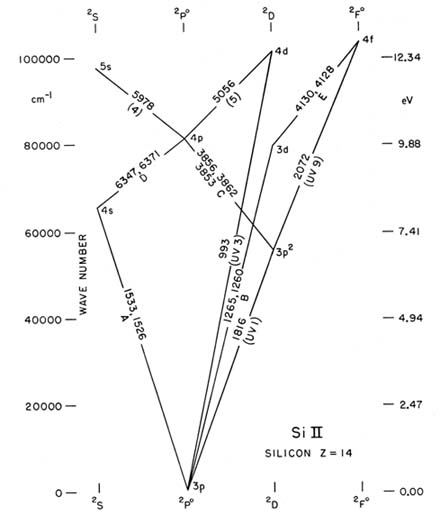
\includegraphics[width=\linewidth]{figures/grotrian-si-ii.jpg}
%\caption{The Grotrian diagram for \ion{Si}{II}.}
%\label{figure:grotrian-si-ii}
%\end{figure}
%The Grotrian diagram for \ion{Si}{II} in Figure~\ref{figure:grotrian-si-ii} shows the
%levels, the permitted transitions, and their wavelengths in
%{\AA}. What are the wavelengths of the resonance lines?
%\end{problem}

%\begin{problem}
%\label{problem-dipole-scattering}
%Show that if the specific intensity is linear in $\mu$, that
%is, $I_\nu = I_0 + \mu I_1$, then the scattered emission
%coefficient resulting from dipole scattering with $g =
%(3/4)(1+\mu_\mathrm{s}^2)$ is isotropic.
%\end{problem}

%\begin{problem} 
%Consider an atmosphere in which the opacity is a mixture of
%pure absorption with an absorption coefficient $\alpha_\nu$
%and coherent electron scattering with a scattering
%coefficient $\sigma_\nu$ and a dipole phase-function
%$g(\mu_\mathrm{s}) = (3/4)(1 + \mu_\mathrm{s}^2)$.

%\begin{enumerate}
%\item[(a)]
%Derive and simplify an expression for the scattered emission
%coefficient $j_\nu^\mathrm{s}(0,\mu)$ at the surface of the
%atmosphere, assuming the source function is given by $S_\nu
%= a_\nu + b_\nu \tau_\nu$.
%\item[(b)]
%Assume that the atmosphere is an LTE grey atmosphere with an
%effective temperature of 10,000 K. Determine the values of
%$S_\nu$ at $\tau_\nu = 0$ and $\tau_\nu = 1$ at 0.5
%{\micron} (using the Eddington approximation that $q \approx
%2/3$) and, making the approximation that $S_\nu \approx
%a_\nu + b_\nu \tau_\nu$, determine the values of $a_\nu$ and
%$b_\nu$.
%\item[(c)] 
%Plot the normalized angular dependence of $j_\nu^\mathrm{s},$
%\begin{align}
%\frac{j_\nu^\mathrm{s}(0,\mu)}{(1/2)\int_{-1}^{+1}\!\!\!d\mu\,j_\nu^\mathrm{s}(0,\mu)
%}
%\end{align}
%at the surface of the atmosphere at this wavelength.
%\item[(d)]
%We can characterize the degree of anisotropy by
%\begin{align}
%\frac{
%j_\nu^\mathrm{s}|_\mathrm{max} - j_\nu^\mathrm{s}|_\mathrm{min}
%}{
%j_\nu^\mathrm{s}|_\mathrm{max} + j_\nu^\mathrm{s}|_\mathrm{min}
%}.
%\end{align}
%What is this characteristic value at the surface of the
%atmosphere at this wavelength?
%\item[(e)]
%By considering the degree of anisotropy, how large does
%$\sigma_\nu$ have to be compared to $\alpha_\nu$ before
%scattering is important at the surface of the atmosphere at
%this wavelength?
%\item[(f)]
%Does anisotropic scattering become more or less important
%deeper in the atmosphere?
%\end{enumerate}
%
%\end{problem}
